% Presentation name and date
% To build, use the following command:
%	NAME="Scopatz_ANSAnnual_2010_Pres" && latex ${NAME}.tex && dvipdf ${NAME}.dvi
\documentclass[pdf, autumn, slideColor, nocolorBG]{prosper}
\usepackage{verbatim}
\usepackage{color}
\usepackage{hyperref}

%General Short-Cut Commands
\newcommand{\superscript}[1]{\ensuremath{^{\textrm{#1}}}}
\newcommand{\subscript}[1]{\ensuremath{_{\textrm{#1}}}}
\newcommand{\nuc}[2]{\superscript{#2}{#1}}
\newcommand{\FigCaption}[1]{\begin{center}{\tiny{#1}}\end{center}}

%Commands for this document...
\newcommand{\Red}[1]{\textcolor{red}{#1}}

%Presentation information
\title{Nuclear Fuel Cycle Sensitivity \& Contingency Table Analysis}
\subtitle{June 15\superscript{th}, 2010 - ANS Annual Meeting\\
San Diego, CA}
\author{Anthony Scopatz\superscript{A}, Jun Li\superscript{B}, 
    Man-Sung Yim\superscript{C}, \& Erich Schneider\superscript{A}}
\email{scopatz@mail.utexas.edu}
\institution{\tiny
\textbf{\underline{A:}}
Department of Mechanical Engineering, Nuclear Engineering Program\\
The University of Texas at Austin\\
1 University Station, MC R9000, Austin, TX 78712\\

\textbf{\underline{B:}}Institute for the Environment\\
The University of North Carolina � Chapel Hill\\
Campus Box 6116, Chapel Hill, NC 27599-6116\\

\textbf{\underline{C:}}
Department of Nuclear Engineering\\
North Carolina State University, Raleigh, NC 27695
}

\slideCaption{Scopatz, \emph{et al.} - ANS Annual 2010}

\begin{document}

% make the title slide
\maketitle


%Motivation
\overlays{5}{
\begin{slide}{Motivation}
\FromSlide{1}
\begin{itemize}
    \item Many nuclear fuel cycle simulations are formulated on premade base-case scenarios:

\FromSlide{2}
    \begin{center}
    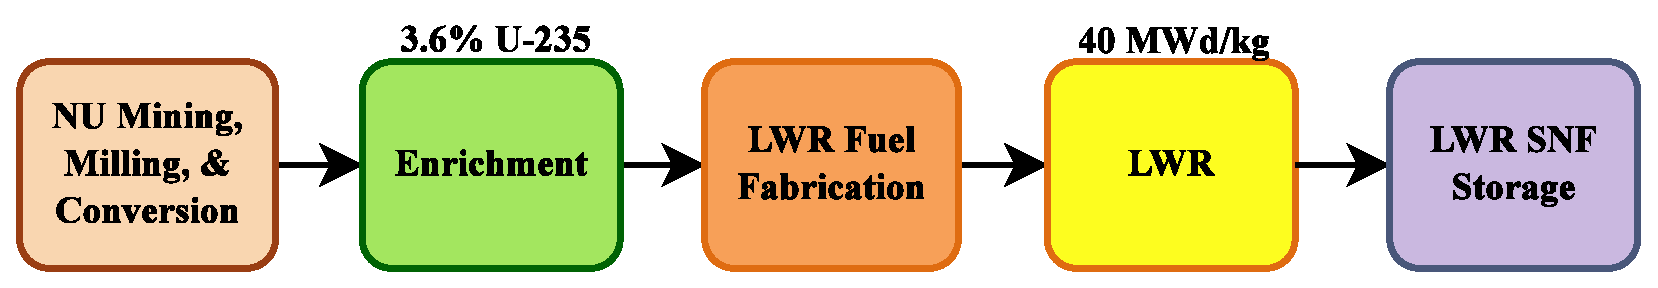
\includegraphics[scale=0.25]{figs/OnceThrough.eps}
    \end{center}

\FromSlide{3}
    \item These base cases are very well studied.

\FromSlide{4}
    \item However, what is \textbf{\textit{not}} well known is 
        how these sample scenarios are affected by perturbations to their 
        initial physical parameters.
            
\FromSlide{1}
\end{itemize}

\FromSlide{5}
\begin{center}
``\textit{Do our parameter choices really give us the `best' solution?}''
\end{center}

\end{slide}}



%Methodology Overview
\overlays{4}{
\begin{slide}{Methodology Overview}
\FromSlide{1}
\begin{itemize}
    \item Here, we quantify the system-wide impact of physical parameter perturbations.

\FromSlide{2}
    \item This is done by performing \textbf{Contingency Table} analysis for each parameter
        to the \underline{repository} \underline{capacity} response, measured in units of energy.  

\FromSlide{3}
    \item Denote fuel cycle responses as $R$ [GWh] for $x$ input parameters.

\FromSlide{4}
    \item \textbf{\underline{Goal:}} Determine strength of association 
        between inputs and pairs of inputs to the response in a manner that is independent to:
        \begin{itemize}
            \item the functional form of the response to the input $R(x)$,
            \item any base-case set of initial inputs.
        \end{itemize}

\FromSlide{1}
\end{itemize}
\end{slide}}


%Background
\overlays{2}{
\begin{slide}{Background}
\FromSlide{1}
We have developed a physics-based fuel cycle model
and used it to study a Fast Reactor (FR), Light
Water Reactor (LWR) symbiotic scenario 
analogous to Scheme 3a of the 2006 OECD report.

\FromSlide{2}
\begin{center}
\includegraphics[scale=0.25]{figs/LWR_FR.eps}
\FigCaption{Figure 1: FR-LWR Cycle}
\end{center}
\end{slide}}



%Background
\overlays{3}{
\begin{slide}{Background}
\FromSlide{1}
\begin{itemize}
    \item In our model, we may adjust over 30 independent physical 
        parameters in the fuel cycle.
\end{itemize}

\FromSlide{2}
\begin{center}
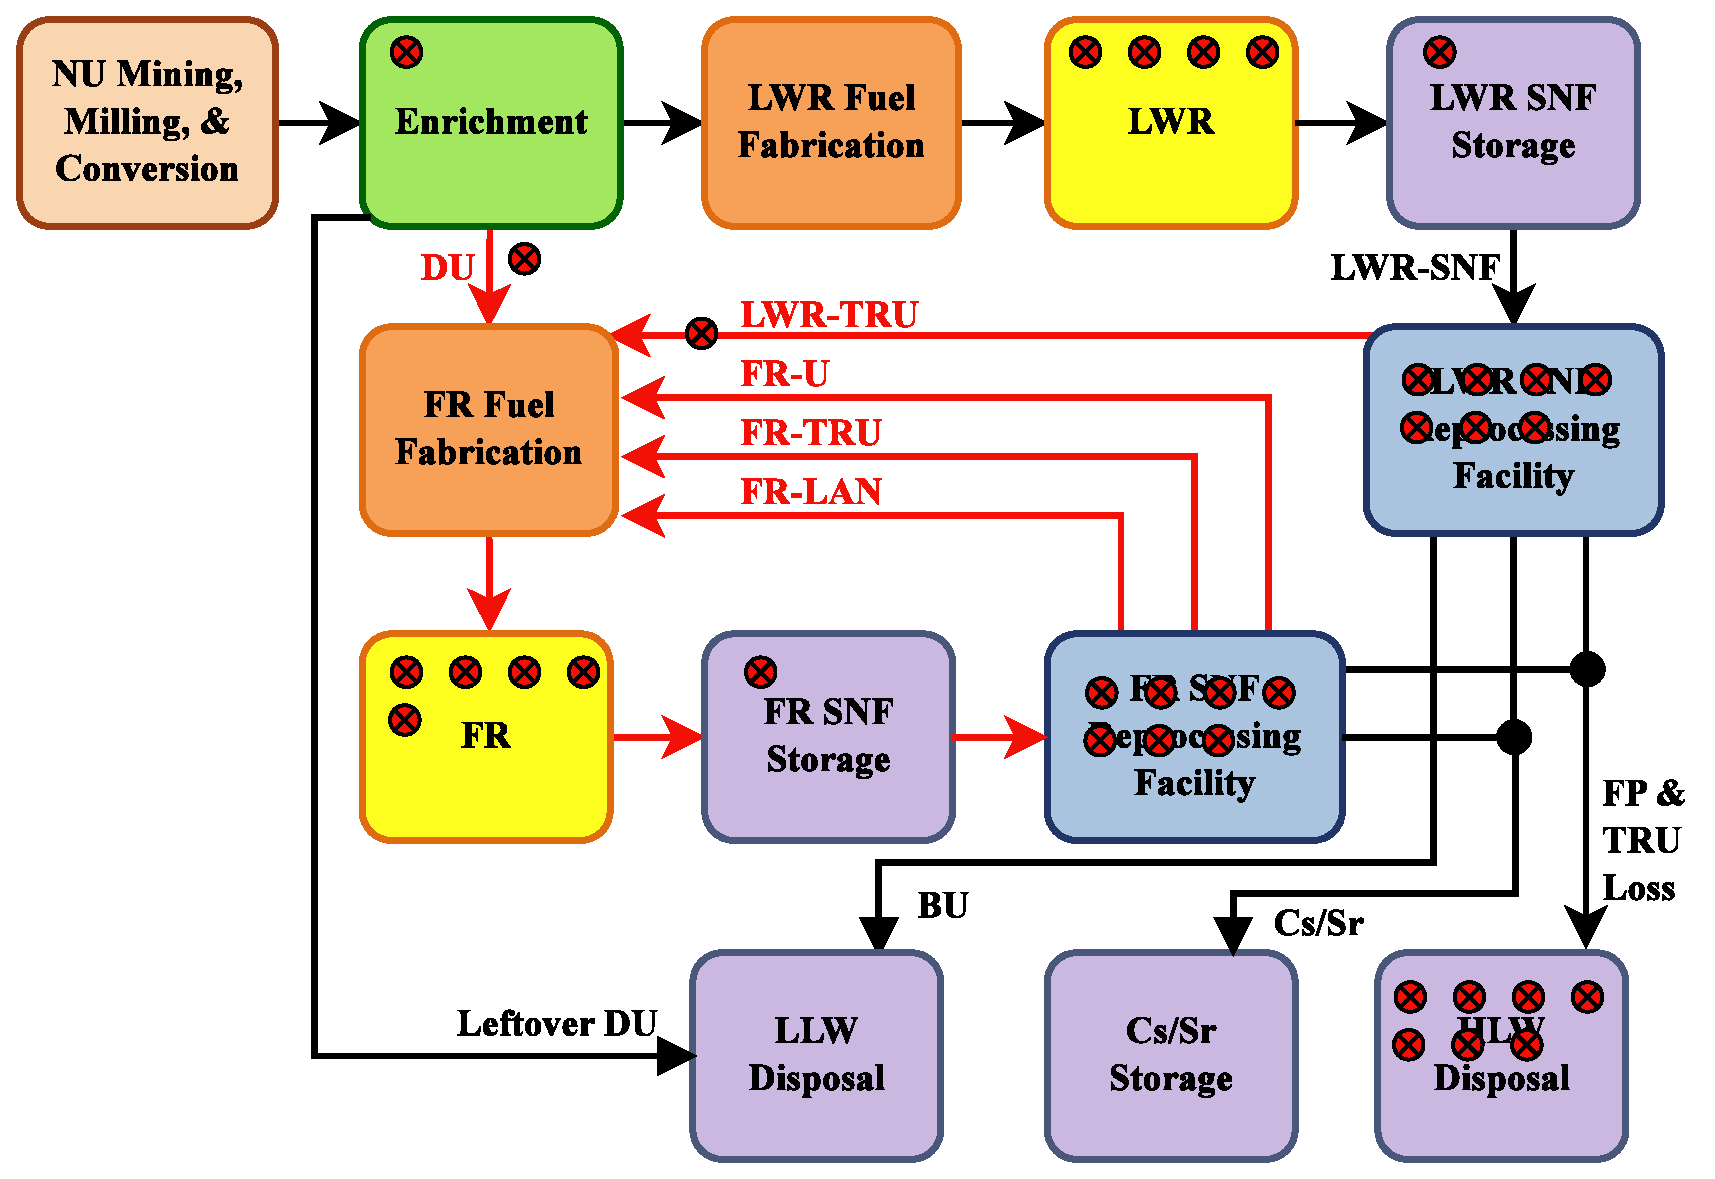
\includegraphics[scale=0.20]{figs/LWR_FR_knobs.eps}
\FigCaption{Figure 2: FR-LWR Cycle with Parameter Representation}
\end{center}

\FromSlide{3}
\begin{itemize}
    \item We present equilibrium results derived from a full treatment
        of the preceding, transient cycles.
\end{itemize}

\end{slide}}


%Fuel Cycle Benchmark
\overlays{4}{
\begin{slide}{Fuel Cycle Benchmark}
\FromSlide{1}
\begin{itemize}
    \item We have benchmarked the model on three primary levels: the reactor components, 
        the repository component, and the fuel cycle as a whole.

\FromSlide{2}
    \item LWRs and FRs benchmarks may be found at 
        {\tiny \url{http://nukestar.me.utexas.edu/scopatz/Bright/}}

\FromSlide{3}
    \item For benchmarks of repository performance, see [1].

\FromSlide{4}
    \item However, since the fuel cycle we are modeling is based off of
        the NEA Scheme 3a, we compared our code to the OECD's own results [2].

\FromSlide{1}
\end{itemize}

\FromSlide{4}
\tiny
\textcolor{gray}{\underline{1:} Li, J., Nicholson, M., Proctor,W.C., Yim, M.-S., McNelis, D.N., 2007. 
``\textit{Examining repository loading options to expand yucca mountain repository capacity.}'' 
In: Proc. Advanced Nuclear Fuel Cycles and Systems, GLOBAL, Boise, ID, September.}

\textcolor{gray}{\underline{2:} Nuclear Energy Agency, ``\textit{Advanced Nuclear Fuel 
Cycles and Radioactive Waste Management,}'' - NEA-5990. 2006:1-248.}
\end{slide}}


%Fuel Cycle Benchmark
\begin{slide}{Fuel Cycle Benchmark}
\tiny
\begin{center}
\FigCaption{Table 1: NEA Scheme 3a Benchmark}
\begin{tabular}{|l||c||c|c||c|c|}
\hline
\textbf{Scheme 3a}     & \textbf{NEA} & \textbf{Model\superscript{1}} & \textbf{\% Diff} & \textbf{Model\superscript{2}} & \textbf{\% Diff} \\
\hline
Electricity Share: LWR & 0.632       & 0.619459             & -2.0244 & 0.634907             & +0.4579 \\
\hline
Electricity Share: FR  & 0.368       & 0.380541             & +3.2955 & 0.365093             & -0.7962 \\
\hline
FR SNF: U              & 0.698       & 0.713806             & +2.2143 & 0.715224             & +2.4082 \\
\hline
FR SNF: NP             & 0.0065      & 0.00661961           & +1.8070 & 0.00685174           & +5.1335 \\
\hline
FR SNF: PU             & 0.266       & 0.248059             & -7.2327 & 0.248319             & -7.1204 \\
\hline
FR SNF: AM             & 0.02        & 0.0226796            & 11.8152 & 0.0217317            & +7.9687 \\
\hline
FR SNF: CM             & 0.0098      & 0.00883517           & -10.920 & 0.00787319           & -24.4730\\
\hline
HLW: U                 & 0.013324    & 0.0132681            & -0.4213 & 0.0134448            & +0.8984 \\
\hline
HLW: NP                & 2.26542E-05 & 2.4079E-05           & +5.9173 & 2.41083E-05          & +6.0316 \\
\hline
HLW: PU                & 0.000704797 & 0.000658893          & -6.9668 & 0.000632361          & -11.4548\\
\hline
HLW: AM                & 5.03426E-05 & 5.63068E-05          & 10.5923 & 5.12344E-05          & +1.7405 \\
\hline
HLW: CM                & 2.18151E-05 & 1.99031E-05          & -9.6068 & 1.67094E-05          & -30.5563\\
\hline
HLW: FP                & 0.985876    & 0.985973             & +0.0098 & 0.985831             & -0.0046 \\
\hline
\end{tabular}
\end{center}

1: Model with initial LWR \nuc{U}{235} enrichment of 4.2 w/o. 

2: Model with LWR discharge burnup of 50 MWd/kg.
\end{slide}




%Analysis Methodology
\overlays{5}{
\begin{slide}{Analysis Methodology}
\FromSlide{1}
\begin{itemize}
    \item Before attempting to comprehend the subtleties of a 30+ dimensional surface,  
        prudence demands that we check and see if we really need all 30 variables...

\FromSlide{2}
    \begin{itemize}
        \item (Hint: we probably don't!)
    \end{itemize}

\FromSlide{3}
    \item Thus we are looking for a quantitative ranking of the \emph{associations} of each input parameter to the response.  

\FromSlide{4}
    \begin{itemize}
        \item (Note that these associations do not imply a linear response!)
    \end{itemize}

\FromSlide{5}
    \item To do this, we are going to borrow an analysis tool that is often used in Biology: \underline{Contingency Tables}.

\FromSlide{1}
\end{itemize}
\end{slide}}



%Contingency Tables
\overlays{3}{
\begin{slide}{Contingency Tables}
\FromSlide{1}
The $2\times 2$ table is most common:
\begin{center}
\FigCaption{Table 2: Hair Color to Sex Contingency Table}
\begin{tabular}{|l||c|c||c|}
\hline
       & Blonde & Brunette & Totals \\
\hline
Female & 18     & 17       & 35 \\
\hline
Male   & 11     & 14       & 25 \\
\hline
Totals & 29     & 31       & 60 \\
\hline
\end{tabular}
\end{center} 

\FromSlide{2}
\vspace{1.0cm}
But doesn't this approach ignore the underlying biology?

\FromSlide{3}
\vspace{1.0cm}
\raggedleft{\LARGE \textit{Yes!}}
\end{slide}}


%Contingency Tables
\begin{slide}{Contingency Tables}
\begin{center}
\includegraphics[scale=0.125]{figs/CTBlackBox/CTBlackBox01.eps}
\end{center}
\end{slide}

%Contingency Tables
\begin{slide}{Contingency Tables}
\begin{center}
\includegraphics[scale=0.125]{figs/CTBlackBox/CTBlackBox02.eps}
\end{center}
\end{slide}


%Contingency Tables
\begin{slide}{Contingency Tables}
\begin{center}
\includegraphics[scale=0.125]{figs/CTBlackBox/CTBlackBox03.eps}
\end{center}
\end{slide}


%Contingency Tables
\begin{slide}{Contingency Tables}
\begin{center}
\includegraphics[scale=0.125]{figs/CTBlackBox/CTBlackBox04.eps}
\end{center}
\end{slide}


%Contingency Tables
\begin{slide}{Contingency Tables}
\begin{center}
\includegraphics[scale=0.125]{figs/CTBlackBox/CTBlackBox05.eps}
\end{center}
\end{slide}


%Contingency Tables
\begin{slide}{Contingency Tables}
\begin{center}
\includegraphics[scale=0.125]{figs/CTBlackBox/CTBlackBox06.eps}
\end{center}
\end{slide}



%Fuel Cycle Contingency Table
\overlays{2}{
\begin{slide}{Fuel Cycle Contingency Table}
\FromSlide{1}
For example, let's construct a 2D contingency table that 
measures the response from a sample input: fast reactor 
fuel plutonium separation efficiency, \texttt{FR\_SE\_PU}.

\FromSlide{2}
\vspace{1.0cm}
\tiny
\FigCaption{Table 3: Contingency Table for \texttt{FR\_SE\_PU} to Repository Capacity.}
\begin{center}
\begin{tabular}{|c||c|c|c||c|}
\hline
&$0.9<$\texttt{SE}$<0.99$&$0.99<$\texttt{SE}$<0.999$&$0.999<$\texttt{SE}$<0.9999$&\\
\hline
$5E08<$R$<5E09$&$1188$&$33$&$26$&$1247$\\
\hline
$5E09<$R$<5E10$&$30010$&$18647$&$16542$&$65199$\\
\hline
$5E10<$R$<5E11$&$3699$&$15877$&$16890$&$36466$\\
\hline
$5E11<$R$<5E12$&$0$&$405$&$1521$&$1926$\\
\hline
&$34897$&$34962$&$34979$&$104838$\\
\hline
\end{tabular}
\end{center}

\end{slide}}


%Input Variable Definition
\begin{slide}{Input Variable Definition}
\tiny
\begin{center}
\begin{tabular}{|l||c|c|c|c|}
\hline
\textbf{Input Paramter $x$} & \textbf{Min} & \textbf{Max} & \textbf{Units} & \textbf{Sample Type}\\
\hline
LWR Burnup Level & 30.0 & 80.0 & MWd/kgIHM & linear \\
\hline
LWR Fuel to Moderator Ratio & 0.28 & 0.36 & & linear \\
\hline
LWR SNF Storage Time & 3 & 30 & years & linear \\
\hline
SE of U from LWR SNF & 0.99 & 0.9999 & & nines \\
\hline
SE of NP from LWR SNF & 0.9 & 0.9999 & & nines \\
\hline
SE of PU from LWR SNF & 0.9 & 0.9999 & & nines \\
\hline
SE of AM from LWR SNF & 0.9 & 0.9999 & & nines \\
\hline
SE of CM from LWR SNF & 0.9 & 0.9999 & & nines \\
\hline
SE of CS from LWR SNF & 0.9 & 0.9999 & & nines \\
\hline
SE of SR from LWR SNF & 0.9 & 0.9999 & & nines \\
\hline
FR Burnup Level & 100.0 & 200.0 & MWd/kgIHM & linear\\
\hline
FR TRU Conversion Ratio & 0.25 & 0.95 & & linear \\
\hline
Max Fraction of Lanthanide in FR Fuel & 0.0001 & 0.005 & Atoms/TRU Atom & linear \\
\hline
FR SNF Storage Time & 3 & 30 & years & linear \\
\hline
Storage Before Disposal & 1 & 300 & years & log \\
\hline
\end{tabular}
\end{center}
\end{slide}

%Input Variable Definition
\begin{slide}{Input Variable Definition}
\tiny
\begin{center}
\begin{tabular}{|l||c|c|c|c|}
\hline
\textbf{Input Paramter $x$} & \textbf{Min} & \textbf{Max} & \textbf{Units} & \textbf{Sample Type}\\
\hline
SE of U from FR SNF & 0.99 & 0.9999 & & nines \\
\hline
SE of NP from FR SNF & 0.9 & 0.9999 & & nines \\
\hline
SE of PU from FR SNF & 0.9 & 0.9999 & & nines \\
\hline
SE of AM from FR SNF & 0.9 & 0.9999 & & nines \\
\hline
SE of CM from FR SNF & 0.9 & 0.9999 & & nines \\
\hline
SE of CS from FR SNF & 0.9 & 0.9999 & & nines \\
\hline
SE of SR from FR SNF & 0.9 & 0.9999 & & nines \\
\hline
Density of Host Rock & 2317 & 2869 & kg/m\superscript{3} & linear \\
\hline
Specific Heat of Host Rock & 590 & 1270 & J/kg-K & linear \\
\hline
Thermal Conductivity of Host Rock & 1.9204 & 3.2856 & W/m-K & linear \\
\hline
Heat Loss Factor During Ventilation  & 0.806 & 0.914 & & linear \\
\hline
Drift diameter & 4.5 & 6.5 & m & linear \\
\hline
Ventilation System On Time & 10 & 300 & years & log \\
\hline
Ambient Environment Temperature & 12.82 & 32.82 & C & linear \\
\hline
Distance Between Drifts & 56 & 106 & m & linear \\
\hline
\end{tabular}
\end{center}
\end{slide}

%Contingency Table Statistics
\overlays{3}{
\begin{slide}{Contingency Table Statistics}
\FromSlide{1}
There are several metrics that have been developed to measure 
associations with contingency tables.  

\FromSlide{2}
\vspace{0.5cm}
The measure we will be using is the \emph{Uncertainty Coefficient} $U(x|R)$.

\FromSlide{3}
\vspace{0.5cm}
To calculate $U(x|R)$ we will need, 
\begin{itemize}
    \item The \emph{Entropy} $H(x)$, which is a measure of how evenly the 
        data is spread out in the $x$ parameter.
    \item The \emph{Mutual Information} $I(R,x)$ which states the shared
        value of the $x$ together with $R$. 
\end{itemize}
\end{slide}}


%Contingency Table Statistics
\overlays{3}{
\begin{slide}{Contingency Table Statistics}
\FromSlide{1}
Denote the entries in a contingency table as $N_{ij}$ for the i\superscript{th} response bin
and the j\superscript{th} input bin.

\FromSlide{2}
\vspace{0.5cm}
The probability of landing in a given bin is therefore, 
\[ p_{ij} = \frac{N_{ij}}{N} \] 

\FromSlide{3}
\vspace{0.5cm}
We may then calculate the entropy from, 
\[ H(x) = - \sum_j^J p_{\cdot j} \ln(p_{\cdot j}) \]
\end{slide}}


%Contingency Table Statistics
\overlays{2}{
\begin{slide}{Contingency Table Statistics}
\FromSlide{1}
The mutual information is found via, 
\[ I(R,x) = - \sum_{i,j}^{I,J} p_{ij} \ln\left(\frac{p_{ij}}{p_{i\cdot}\cdot p_{\cdot j}}\right) \]

\FromSlide{2}
\vspace{0.5cm}
The relations may be seen graphically:

\vspace{0.5cm}
\setlength{\unitlength}{1cm}
\begin{center}
\begin{picture}(9,3)(-4.5,-1.5)
\thicklines
\put(0,1.5){\vector(1,0){4.5}}
\put(0,1.5){\vector(-1,0){4.5}}
\put(-0.7,1.2){\tiny $H(x,R)$}

\put(-2.25,1.0){\vector(1,0){2.25}}
\put(-2.25,1.0){\vector(-1,0){2.25}}
\put(-2.6,0.7){\tiny $H(x)$}

\put(1.5,0.5){\vector(1,0){3}}
\put(1.5,0.5){\vector(-1,0){3}}
\put(1.2,0.2){\tiny $H(R)$}

\put(-0.75,0){\vector(1,0){0.75}}
\put(-0.75,0){\vector(-1,0){0.75}}
\put(-1.2,-0.3){\tiny $I(R,x)$}

\put(-3,-0.5){\vector(1,0){1.5}}
\put(-3,-0.5){\vector(-1,0){1.5}}
\put(-3.5,-0.8){\tiny $H(x|R)$}

\put(2.25,-0.5){\vector(1,0){2.25}}
\put(2.25,-0.5){\vector(-1,0){2.25}}
\put(2.0,-0.8){\tiny $H(R|x)$}

\end{picture}
\end{center}

\end{slide}}


%Contingency Table Statistics
\overlays{2}{
\begin{slide}{Contingency Table Statistics}
\FromSlide{1}
The uncertainty coefficient is then calculated from,
\[ U(x|R) = \frac{I(R,x)}{H(x)} \]

\FromSlide{2}
This metric has the following useful properties:
\begin{enumerate}
    \item Defined on the range $0 \to 1$.
    \item $U(x|R) = 0$ implies that $I(R,x) = 0$ which indicates that the parameter
        is unassociated with the response.
    \item $U(x|R) = 1$ means that $I(R,x) = H(R) = H(x)$.  This means
        the system response $R(x)$ is solely determined by $x$.
\end{enumerate}
\end{slide}}



%Contingency Table Statistics
\overlays{2}{
\begin{slide}{Contingency Table Statistics}
\FromSlide{1}
\vspace{1cm}
\begin{minipage}[t]{5.0cm}
\begin{center}
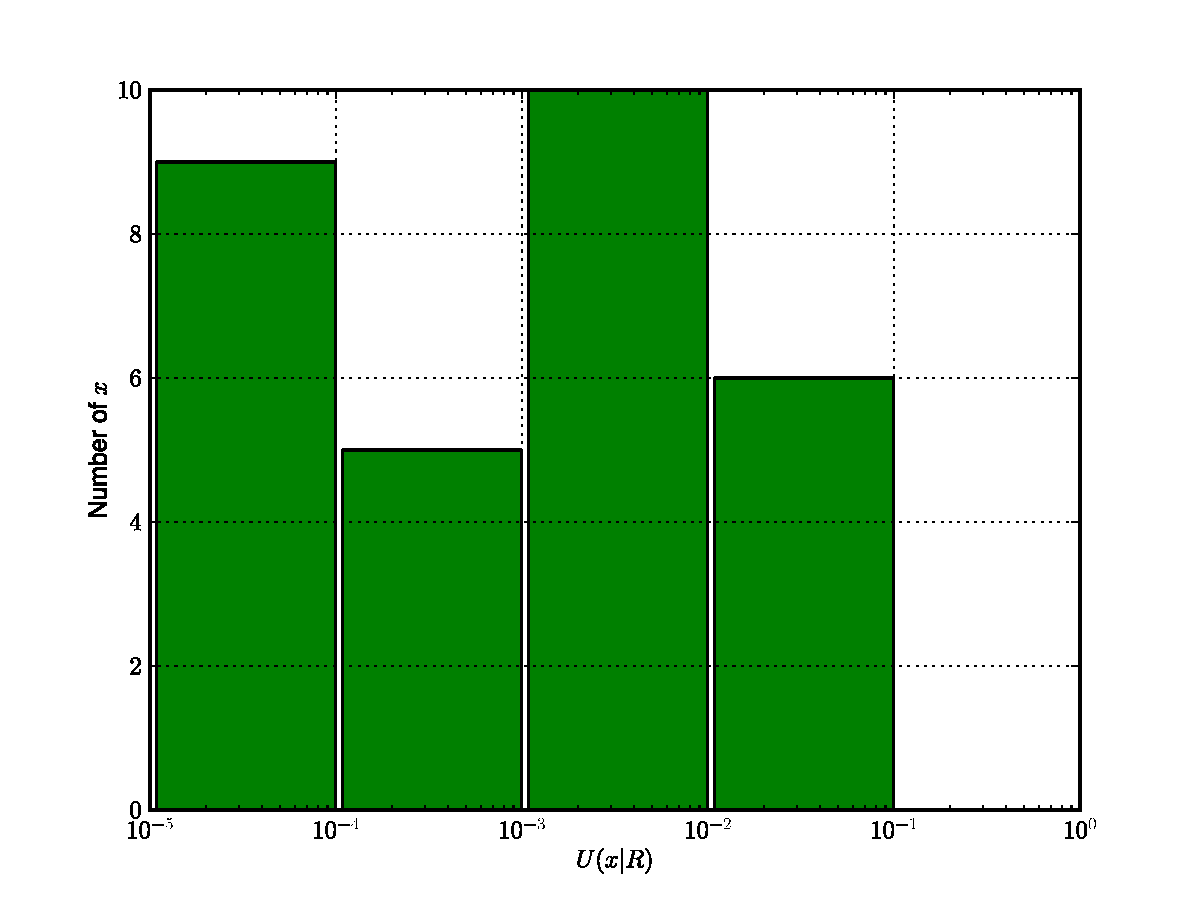
\includegraphics[scale=0.25]{figs/Total_Electricity_2D_U_x_R.eps}
\FigCaption{Fig 3: $U(x|R)$ Histogram for Repository Capacity}
\end{center}
\end{minipage}
\FromSlide{2}
\begin{minipage}[t]{5cm}
\tiny
\begin{center}
\FigCaption{Table 4: Top Parameters Affecting Repository Capacity}
\begin{tabular}{|l|c|}
\hline
\textbf{Independent Parameter $x$}&\textbf{$U(x|R)$}\\
\hline
\texttt{FR\_SE\_PU}             &0.0862\\
\hline
\texttt{INT\_SNF\_Storage\_Time}&0.0598\\
\hline
\texttt{FR\_SE\_AM}             &0.0436\\
\hline
\texttt{Heat\_Loss\_Factor}     &0.0161\\
\hline
\texttt{LWR\_SE\_PU}            &0.0131\\
\hline
\texttt{FR\_TRU\_CR}            &0.0101\\
\hline
\end{tabular}
\end{center}

\end{minipage}
\end{slide}}



%Contingency Table Extensions
\overlays{5}{
\begin{slide}{Contingency Table Extensions}
\FromSlide{1}
\begin{itemize}
    \item \textbf{\underline{New Goal:}} Now that we are able to determine the assoction of $x$ to $R$, we 
        should be able to find the sensitivity of $R(x)$ to other inputs.

\FromSlide{2}
    \item Call $y$ an input parameter distinct from $x$.  We can then measure the simultaneous 
        effect of two inputs to the response using 3D tables! 

\FromSlide{3}
    \item Note that \textit{`slices'} of this 3D table may be seen as 2D tables bins along a specific cut of data.

\FromSlide{4}
    \item As we have 30 inputs, there are now $_{30}C_2 = 435$ contingency tables we must construct.

\FromSlide{5}
    \item Naturally, different metrics will be needed to account for the added dimensionality.

\FromSlide{1}
\end{itemize}
\end{slide}}


%Table 5: 3D Contingency Table
\begin{slide}{Table 5: 3D Contingency Table}
\begin{center}
\tiny
\FigCaption{Slice for 10 $<$ \texttt{Vent\_System\_On\_Time} $<$ 31.0723}
\begin{tabular}{|c||c|c|c||c|}
\hline
&$0.9<$\texttt{SE}$<0.99$&$0.99<$\texttt{SE}$<0.999$&$0.999<$\texttt{SE}$<0.9999$&\\
\hline
$5E08<$R$<5E09$&$420$&$8$&$7$&$435$\\
\hline
$5E09<$R$<5E10$&$9987$&$6153$&$5538$&$21678$\\
\hline
$5E10<$R$<5E11$&$1227$&$5289$&$5665$&$12181$\\
\hline
$5E11<$R$<5E12$&$0$&$121$&$507$&$628$\\
\hline
&$11634$&$11571$&$11717$&$34922$\\
\hline
\end{tabular}
\end{center}

\vspace{0.75cm}

\begin{center}
\tiny
\FigCaption{Slice for 31.0723 $<$ \texttt{Vent\_System\_On\_Time} $<$ 96.5489}
\begin{tabular}{|c||c|c|c||c|}
\hline
&$0.9<$\texttt{SE}$<0.99$&$0.99<$\texttt{SE}$<0.999$&$0.999<$\texttt{SE}$<0.9999$&\\
\hline
$5E08<$R$<5E09$&$397$&$8$&$9$&$414$\\
\hline
$5E09<$R$<5E10$&$10063$&$6185$&$5472$&$21720$\\
\hline
$5E10<$R$<5E11$&$1219$&$5332$&$5612$&$12163$\\
\hline
$5E11<$R$<5E12$&$0$&$151$&$496$&$647$\\
\hline
&$11679$&$11676$&$11589$&$34944$\\
\hline
\end{tabular}
\end{center}
\end{slide}


%Table 5: 3D Contingency Table
\begin{slide}{Table 5: 3D Contingency Table}
\begin{center}
\tiny
\FigCaption{Slice for 96.5489 $<$ \texttt{Vent\_System\_On\_Time} $<$ 300}
\begin{tabular}{|c||c|c|c||c|}
\hline
&$0.9<$\texttt{SE}$<0.99$&$0.99<$\texttt{SE}$<0.999$&$0.999<$\texttt{SE}$<0.9999$&\\
\hline
$5E08<$R$<5E09$&$371$&$17$&$10$&$398$\\
\hline
$5E09<$R$<5E10$&$9960$&$6309$&$5532$&$21801$\\
\hline
$5E10<$R$<5E11$&$1253$&$5256$&$5613$&$12122$\\
\hline
$5E11<$R$<5E12$&$0$&$133$&$518$&$651$\\
\hline
&$11584$&$11715$&$11673$&$34972$\\
\hline
\end{tabular}
\end{center}

\vspace{0.75cm}

\begin{center}
\tiny
\FigCaption{Summary for summation over \texttt{Vent\_System\_On\_Time}}
\begin{tabular}{|c||c|c|c||c|}
\hline
&$0.9<$\texttt{SE}$<0.99$&$0.99<$\texttt{SE}$<0.999$&$0.999<$\texttt{SE}$<0.9999$&\\
\hline
$5E08<$R$<5E09$&$1188$&$33$&$26$&$1247$\\
\hline
$5E09<$R$<5E10$&$30010$&$18647$&$16542$&$65199$\\
\hline
$5E10<$R$<5E11$&$3699$&$15877$&$16890$&$36466$\\
\hline
$5E11<$R$<5E12$&$0$&$405$&$1521$&$1926$\\
\hline
&$34897$&$34962$&$34979$&$104838$\\
\hline
\end{tabular}
\end{center}
\end{slide}


%3D Contingency Table Statistics
\overlays{2}{
\begin{slide}{3D Contingency Table Statistics}
\FromSlide{1}
To gauge the \textit{total} strength of association of two parameters together to a response, 
we use a 3D version of the uncertainty coefficient:
\[ U(x,y|R) = \frac{I(R,x,y)}{H(x,y)} \]

\FromSlide{2}
Likewise, this metric has the following properties:
\begin{enumerate}
    \item Defined on the range $0 \to 1$.
    \item $U(x,y|R) = 0$ implies that $I(R,x) = 0$ and that the parameters
        is do not affect the response.
    \item $U(x,y|R) = 1$ means that $H(R) = H(x) = H(y)$  and
        $R(x,y,\ldots)$ is solely determined by $x$ and $y$.
\end{enumerate}
\end{slide}}


%$U(x,y|R)$ Top Parameter Pairs
\begin{slide}{$U(x,y|R)$ Top Parameter Pairs}
\tiny
\begin{center}
\FigCaption{Table 6: Top Parameter Pairs Affecting Repository Capacity}
\begin{tabular}{|l|l|c|}
\hline
\textbf{Independent Parameter $x$}&\textbf{Independent Parameter $y$}&\textbf{$U(x,y|R)$}\\
\hline
\texttt{FR\_SE\_PU}&\texttt{Cooling\_Time}               & 0.0786\\
\hline
\texttt{FR\_SE\_AM}&\texttt{FR\_SE\_PU}                  & 0.0688\\
\hline
\texttt{FR\_SE\_AM}&\texttt{INT\_SNF\_Storage\_Time}     & 0.0547\\
\hline
\texttt{FR\_SE\_PU}&\texttt{Heat\_Loss\_Factor}          & 0.0526\\
\hline
\texttt{FR\_SE\_PU}&\texttt{LWR\_SE\_PU}                 & 0.0505\\
\hline
\texttt{FR\_SE\_PU}&\texttt{FR\_TRU\_CR}                 & 0.0492\\
\hline
\texttt{FR\_SE\_PU}&\texttt{LWR\_SE\_U}                  & 0.0482\\
\hline
\texttt{FR\_SE\_PU}&\texttt{LWR\_SE\_AM}                 & 0.0467\\
\hline
\texttt{FR\_SE\_PU}&\texttt{LWR\_SNF\_Storage\_Time}     & 0.0449\\
\hline
\texttt{FR\_SE\_PU}&\texttt{Rock\_Specific\_Heat}        & 0.0448\\
\hline
\texttt{FR\_SE\_CM}&\texttt{FR\_SE\_PU}                  & 0.0445\\
\hline
\texttt{FR\_BUd}&\texttt{FR\_SE\_PU}                     & 0.0444\\
\hline
\texttt{FR\_SE\_PU}&\texttt{LWR\_BUd}                    & 0.0443\\
\hline
\texttt{FR\_SE\_PU}&\texttt{Rock\_Thermal\_Conductivity} & 0.0442\\
\hline
\end{tabular}
\end{center}

\begin{comment}
\texttt{Ambient\_Temp}&\texttt{FR\_SE\_PU}&0.0438545730185\\
\hline
\texttt{FR\_SE\_PU}&\texttt{LWR\_SE\_CS}&0.0438481227943\\
\hline
\texttt{FR\_SE\_PU}&\texttt{LWR\_SE\_SR}&0.0436468041277\\
\hline
\texttt{Drift\_Space}&\texttt{FR\_SE\_PU}&0.0434940997611\\
\hline
\texttt{FR\_SE\_PU}&\texttt{FR\_SNF\_Storage\_Time}&0.0433708807088\\
\hline
\texttt{FR\_SE\_CS}&\texttt{FR\_SE\_PU}&0.0432348364514\\
\hline
\texttt{FR\_SE\_PU}&\texttt{Rock\_Density}&0.043203201625\\
\hline
\texttt{FR\_SE\_PU}&\texttt{LWR\_SE\_CM}&0.0431931733916\\
\hline
\end{comment}


\end{slide}



%3D Contingency Table Statistics
\overlays{4}{
\begin{slide}{3D Contingency Table Statistics}
\FromSlide{1}
\begin{itemize}
    \item If $U(x,y|R)$ is roughly equivalent to the concept of \textit{mutual} \textit{sensitivity}, 
        then the 3D tables should allow for an information theoretic parallel to \textit{\underline{covariance}}!

\FromSlide{2}
    \item In general for contingency tables this is likely not true, but here we are in the special stochastic 
        situation where we know \textit{a priori} $x$ and $y$ to be independent from $R$.

\FromSlide{3}
    \item Therefore, we propose the following metric:

\FromSlide{4}
        \begin{itemize}
            \item $S(x,y)$ measures \textit{relative} sensitivity for 2+ inputs to the response.

%\FromSlide{5}
%            \item $U(x|R,y)$ is the `sensitivity of sensitivities', or how much an input 
%                affects both the response and the value of another input.
%        
%\FromSlide{4}
        \end{itemize}

\FromSlide{1}
\end{itemize}
\end{slide}}




%3D Contingency Table Statistics
\overlays{2}{
\begin{slide}{3D Contingency Table Statistics}
\FromSlide{1}
$S$ is defined as:
\[ S(x,y) = 1 - \frac{U(x|R) + U(y|R)}{2U(x,y|R)} \]

\FromSlide{2}
Thus, $S$ has the following properties:
\begin{enumerate}
    \item Defined on the range $0 \to 1$.
    \item $S = 0$: Response solely determined by one variable. Second variable contribution irrelevant.
    \item $S < 1$: Response is determined by combination of both variables, though one independent 
        parameter shows a weaker dependence.
    \item $S = 1$: Response is perfectly determined by both variables in tandem.
\end{enumerate}
\end{slide}}


\begin{comment}
%3D Contingency Table Statistics
\overlays{2}{
\begin{slide}{3D Contingency Table Statistics}
\FromSlide{1}
$U(x|R,y)$ is defined as:
\[ U(x|R,y) = \frac{I(R,x,y)}{H(x)} \]

\FromSlide{2}
$U(x|R,y)$ has the following properties:
\begin{enumerate}
    \item Defined on the range $0 \to 1$.
    \item $U(x|R,y) = 0$: Perfectly entropic; $x$ does not determine anything about the system.
    \item $U(x|R,y) < 1$: $R$ shows some dependence on $y$ and $R(y)$ in turn shows some dependence on $x$.
    \item $U(x|R,y) = 1$: $x$ exactly determines $R$ and $y$ exactly determines $R$.
\end{enumerate}
\end{slide}}
\end{comment}



%$S(x,y)$
\begin{slide}{$S(x,y)$}
\begin{center}
\FigCaption{Fig 4: Repository Capacity $S(x,y)$ Histogram}
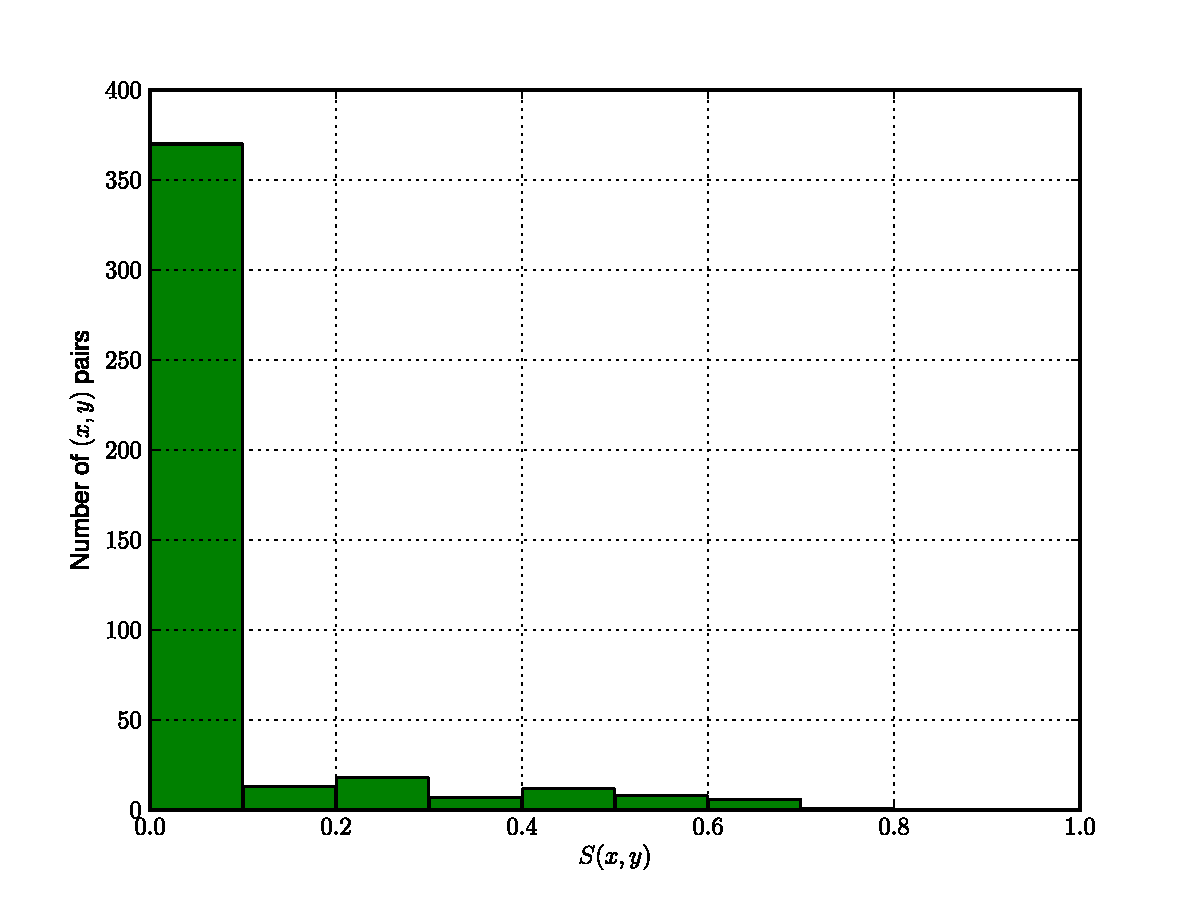
\includegraphics[scale=0.5]{figs/Total_Electricity_3D_S.eps}
\end{center}
\end{slide}




%Parameter Pair Sensitivities
\begin{slide}{Parameter Pair Sensitivities}
\tiny
\FigCaption{Table 7: Parameter Pair Sensitivity Affects to Repository Capacity, Screened by $0.001 < U(x,y|R)$}
\begin{center}
\begin{tabular}{|l|l|c|c|}
\hline
\textbf{Independent Parameter $x$}&\textbf{Independent Parameter $y$}&\textbf{$S(x,y)$}\\
\hline
\texttt{LWR\_Fuel2Mod}&\texttt{Rock\_Thermal\_Conductivity}&0.0869\\
\hline
\texttt{LWR\_SE\_AM}&\texttt{LWR\_SNF\_Storage\_Time}&0.08155\\
\hline
\texttt{FR\_SE\_PU}&\texttt{Cooling\_Time}&0.07187\\
\hline
\texttt{FR\_SE\_CM}&\texttt{FR\_SNF\_Storage\_Time}&0.0713\\
\hline
\texttt{Cooling\_Time}&\texttt{LWR\_SNF\_Storage\_Time}&0.06989\\
\hline
\texttt{FR\_SE\_U}&\texttt{Rock\_Thermal\_Conductivity}&0.06714\\
\hline
\texttt{FR\_SE\_AM}&\texttt{FR\_SE\_PU}&0.05621\\
\hline
\texttt{FR\_SE\_AM}&\texttt{Cooling\_Time}&0.05508\\
\hline
\texttt{FR\_SE\_AM}&\texttt{FR\_TRU\_CR}&0.05075\\
\hline
\texttt{FR\_LAN\_FF\_Cap}&\texttt{LWR\_BUd}&0.046\\
\hline
\texttt{FR\_BUd}&\texttt{LWR\_SE\_SR}&0.04452\\
\hline
\texttt{LWR\_BUd}&\texttt{LWR\_SE\_CM}&0.04396\\
\hline
\texttt{FR\_SE\_CM}&\texttt{LWR\_SE\_NP}&0.04381\\
\hline
\texttt{LWR\_BUd}&\texttt{LWR\_SE\_CS}&0.04345\\
\hline
\end{tabular}
\end{center}


\begin{comment}
\texttt{Ambient\_Temp}&\texttt{FR\_SE\_CM}&0.04092\\
\hline
\texttt{FR\_SE\_U}&\texttt{LWR\_BUd}&0.03978\\
\hline
\texttt{LWR\_SE\_SR}&\texttt{Rock\_Thermal\_Conductivity}&0.03934\\
\hline
\texttt{Ambient\_Temp}&\texttt{Rock\_Thermal\_Conductivity}&0.03814\\
\hline
\texttt{FR\_BUd}&\texttt{FR\_SNF\_Storage\_Time}&0.03783\\
\hline
\texttt{Heat\_Loss\_Factor}&\texttt{Cooling\_Time}&0.03696\\
\hline
\texttt{LWR\_BUd}&\texttt{LWR\_SE\_NP}&0.0363\\
\hline
\texttt{LWR\_SNF\_Storage\_Time}&\texttt{Rock\_Thermal\_Conductivity}&0.03601\\
\hline
\end{comment}

\end{slide}




%Parameter Pair Examples
\overlays{5}{
\begin{slide}{Parameter Pair Examples}
\FromSlide{1}
\begin{itemize}
    \item To get a better grasp on the physical meaning of $S(x,y)$, it is helpful to 
        look at an illustration related to Table 7.

\FromSlide{2}
    \item Take \texttt{FR\_SE\_SR} and \texttt{FR\_SE\_PU}, for example.

\FromSlide{3}
    \item \nuc{Sr}{90} has a half-life of 28.79 years which makes it a medium-term driver of the repository.  

\FromSlide{4}
    Meanwhile, \texttt{FR\_SE\_PU} has the highest overall system impact.

\FromSlide{5}
    \item Because these two inputs are important, it makes intuitive sense that their combined, relative fuel cycle affect is 
        also relatively high at $S = 0.0026$. 

\FromSlide{1}
\end{itemize}
\end{slide}}



%Conclusions
\overlays{4}{
\begin{slide}{Conclusions}
\FromSlide{1}
\begin{itemize}
    \item We have demonstrated a successful and robust alternative to simple fuel cycle sensitivity studies using
        contingency tables and their related statistics.

\FromSlide{2}
    \item This methodology is both quantitative and independent of the functional form between the input and response. 

\FromSlide{3}
    \item In fact, the above does not even require that the stochastic variables be sampled in the same way.

\FromSlide{4}
    \item Future work will involve applying this methodology to more system responses and other statistical metrics.

\FromSlide{1}
\end{itemize}
\end{slide}}


%Questions
\begin{slide}{Questions}
? ? ? ? ? ? ? ? ? ? ? ? ? ? ? ? ? ? ? ? ? ? ? ? ? ? ? ? ? ? ? 
? ? ? ? ? ? ? ? ? ? ? ? ? ? ? ? ? ? ? ? ? ? ? ? ? ? ? ? ? ? ? 
? ? ? ? ? ? ? ? ? ? ? ? ? ? ? ? ? ? ? ? ? ? ? ? ? ? ? ? ? ? ? 
? ? ? ? ? ? ? ? ? ? ? ? ? ? ? ? ? ? ? ? ? ? ? ? ? ? ? ? ? ? ? 
? ? ? ? ? ? ? ? ? ? ? ? ? ? ? ? ? ? ? ? ? ? ? ? ? ? ? ? ? ? ? 
? ? ? ? ? ? ? ? ? ? ? ? ? ? ? ? ? ? ? ? ? ? ? ? ? ? ? ? ? ? ? 
? ? ? ? ? ? ? ? ? ? ? ? ? ? ? ? ? ? ? ? ? ? ? ? ? ? ? ? ? ? ? 
? ? ? ? ? ? ? ? ? ? ? ? ? ? ? ? ? ? ? ? ? ? ? ? ? ? ? ? ? ? ? 
? ? ? ? ? ? ? ? ? ? ? ? ? ? ? ? ? ? ? ? ? ? ? ? ? ? ? ? ? ? ? 
? ? ? ? ? ? ? ? ? ? ? ? ? ? ? ? ? ? ? ? ? ? ? ? ? ? ? ? ? ? ? 
? ? ? ? ? ? ? ? ? ? ? ? ? ? ? ? ? ? ? ? ? ? ? ? ? ? ? ? ? ? ? 
? ? ? ? ? ? ? ? ? ? ? ? ? ? ? ? ? ? ? ? ? ? ? ? ? ? ? ? ? ? ? 
? ? ? ? ? ? ? ? ? ? ? ? ? ? ? ? ? ?
\end{slide}

\end{document}
